\documentclass[]{article}
\usepackage{lmodern}
\usepackage{amssymb,amsmath}
\usepackage{ifxetex,ifluatex}
\usepackage{fixltx2e} % provides \textsubscript
\ifnum 0\ifxetex 1\fi\ifluatex 1\fi=0 % if pdftex
  \usepackage[T1]{fontenc}
  \usepackage[utf8]{inputenc}
\else % if luatex or xelatex
  \ifxetex
    \usepackage{mathspec}
  \else
    \usepackage{fontspec}
  \fi
  \defaultfontfeatures{Ligatures=TeX,Scale=MatchLowercase}
\fi
% use upquote if available, for straight quotes in verbatim environments
\IfFileExists{upquote.sty}{\usepackage{upquote}}{}
% use microtype if available
\IfFileExists{microtype.sty}{%
\usepackage{microtype}
\UseMicrotypeSet[protrusion]{basicmath} % disable protrusion for tt fonts
}{}
\usepackage[margin=1in]{geometry}
\usepackage{hyperref}
\hypersetup{unicode=true,
            pdftitle={Locker-Angelina-ADA-Data-Reanalysis},
            pdfauthor={Angelina Locker},
            pdfborder={0 0 0},
            breaklinks=true}
\urlstyle{same}  % don't use monospace font for urls
\usepackage{color}
\usepackage{fancyvrb}
\newcommand{\VerbBar}{|}
\newcommand{\VERB}{\Verb[commandchars=\\\{\}]}
\DefineVerbatimEnvironment{Highlighting}{Verbatim}{commandchars=\\\{\}}
% Add ',fontsize=\small' for more characters per line
\usepackage{framed}
\definecolor{shadecolor}{RGB}{248,248,248}
\newenvironment{Shaded}{\begin{snugshade}}{\end{snugshade}}
\newcommand{\KeywordTok}[1]{\textcolor[rgb]{0.13,0.29,0.53}{\textbf{#1}}}
\newcommand{\DataTypeTok}[1]{\textcolor[rgb]{0.13,0.29,0.53}{#1}}
\newcommand{\DecValTok}[1]{\textcolor[rgb]{0.00,0.00,0.81}{#1}}
\newcommand{\BaseNTok}[1]{\textcolor[rgb]{0.00,0.00,0.81}{#1}}
\newcommand{\FloatTok}[1]{\textcolor[rgb]{0.00,0.00,0.81}{#1}}
\newcommand{\ConstantTok}[1]{\textcolor[rgb]{0.00,0.00,0.00}{#1}}
\newcommand{\CharTok}[1]{\textcolor[rgb]{0.31,0.60,0.02}{#1}}
\newcommand{\SpecialCharTok}[1]{\textcolor[rgb]{0.00,0.00,0.00}{#1}}
\newcommand{\StringTok}[1]{\textcolor[rgb]{0.31,0.60,0.02}{#1}}
\newcommand{\VerbatimStringTok}[1]{\textcolor[rgb]{0.31,0.60,0.02}{#1}}
\newcommand{\SpecialStringTok}[1]{\textcolor[rgb]{0.31,0.60,0.02}{#1}}
\newcommand{\ImportTok}[1]{#1}
\newcommand{\CommentTok}[1]{\textcolor[rgb]{0.56,0.35,0.01}{\textit{#1}}}
\newcommand{\DocumentationTok}[1]{\textcolor[rgb]{0.56,0.35,0.01}{\textbf{\textit{#1}}}}
\newcommand{\AnnotationTok}[1]{\textcolor[rgb]{0.56,0.35,0.01}{\textbf{\textit{#1}}}}
\newcommand{\CommentVarTok}[1]{\textcolor[rgb]{0.56,0.35,0.01}{\textbf{\textit{#1}}}}
\newcommand{\OtherTok}[1]{\textcolor[rgb]{0.56,0.35,0.01}{#1}}
\newcommand{\FunctionTok}[1]{\textcolor[rgb]{0.00,0.00,0.00}{#1}}
\newcommand{\VariableTok}[1]{\textcolor[rgb]{0.00,0.00,0.00}{#1}}
\newcommand{\ControlFlowTok}[1]{\textcolor[rgb]{0.13,0.29,0.53}{\textbf{#1}}}
\newcommand{\OperatorTok}[1]{\textcolor[rgb]{0.81,0.36,0.00}{\textbf{#1}}}
\newcommand{\BuiltInTok}[1]{#1}
\newcommand{\ExtensionTok}[1]{#1}
\newcommand{\PreprocessorTok}[1]{\textcolor[rgb]{0.56,0.35,0.01}{\textit{#1}}}
\newcommand{\AttributeTok}[1]{\textcolor[rgb]{0.77,0.63,0.00}{#1}}
\newcommand{\RegionMarkerTok}[1]{#1}
\newcommand{\InformationTok}[1]{\textcolor[rgb]{0.56,0.35,0.01}{\textbf{\textit{#1}}}}
\newcommand{\WarningTok}[1]{\textcolor[rgb]{0.56,0.35,0.01}{\textbf{\textit{#1}}}}
\newcommand{\AlertTok}[1]{\textcolor[rgb]{0.94,0.16,0.16}{#1}}
\newcommand{\ErrorTok}[1]{\textcolor[rgb]{0.64,0.00,0.00}{\textbf{#1}}}
\newcommand{\NormalTok}[1]{#1}
\usepackage{graphicx,grffile}
\makeatletter
\def\maxwidth{\ifdim\Gin@nat@width>\linewidth\linewidth\else\Gin@nat@width\fi}
\def\maxheight{\ifdim\Gin@nat@height>\textheight\textheight\else\Gin@nat@height\fi}
\makeatother
% Scale images if necessary, so that they will not overflow the page
% margins by default, and it is still possible to overwrite the defaults
% using explicit options in \includegraphics[width, height, ...]{}
\setkeys{Gin}{width=\maxwidth,height=\maxheight,keepaspectratio}
\IfFileExists{parskip.sty}{%
\usepackage{parskip}
}{% else
\setlength{\parindent}{0pt}
\setlength{\parskip}{6pt plus 2pt minus 1pt}
}
\setlength{\emergencystretch}{3em}  % prevent overfull lines
\providecommand{\tightlist}{%
  \setlength{\itemsep}{0pt}\setlength{\parskip}{0pt}}
\setcounter{secnumdepth}{0}
% Redefines (sub)paragraphs to behave more like sections
\ifx\paragraph\undefined\else
\let\oldparagraph\paragraph
\renewcommand{\paragraph}[1]{\oldparagraph{#1}\mbox{}}
\fi
\ifx\subparagraph\undefined\else
\let\oldsubparagraph\subparagraph
\renewcommand{\subparagraph}[1]{\oldsubparagraph{#1}\mbox{}}
\fi

%%% Use protect on footnotes to avoid problems with footnotes in titles
\let\rmarkdownfootnote\footnote%
\def\footnote{\protect\rmarkdownfootnote}

%%% Change title format to be more compact
\usepackage{titling}

% Create subtitle command for use in maketitle
\newcommand{\subtitle}[1]{
  \posttitle{
    \begin{center}\large#1\end{center}
    }
}

\setlength{\droptitle}{-2em}

  \title{Locker-Angelina-ADA-Data-Reanalysis}
    \pretitle{\vspace{\droptitle}\centering\huge}
  \posttitle{\par}
    \author{Angelina Locker}
    \preauthor{\centering\large\emph}
  \postauthor{\par}
      \predate{\centering\large\emph}
  \postdate{\par}
    \date{April 4, 2019}


\begin{document}
\maketitle

\subsection{Introduction}\label{introduction}

Wright (2012) investigates migration from the ancient Maya site of Tikal
in Guatemala. She presents oxygen and strontium isotopic data from
dental samples from 136 ancient individuals. The individuals included in
her analysis span the Preclassic (400 BCE - 250 CE) to Terminal Classic
(800CE - 900CE) in an attempt to parcel out periods of time where
immigration may have been more prominent than others. Wright (2012)
showcases that approximately 11-16\% of the sampled population were
non-local to the site of Tikal. The majority of these non-local
individuals were high status ``elites'' from the Early Classic (250 -
550 CE); however, ``commoner'' immigrants were identified in household
burials from both the Early and Terminal Classic periods. Wright (2012)
concludes that while Tikal depended on immigration of elites to help
establish their strength as a polity, immigrants from all socioeconimic
backgrounds contributed to the city's expansion and growth.

Wright's (2012) dataset provides contextual information for 134
individuals excavated at Tikal. She provides strontium (Sr) isotope
ratios for 97 individuals and oxygen (O) isotope ratios for 123 of them.
86 individuals have both strontium and oxygen isotope ratios, which is
beneficial to being able to parcel out geographic differences in
instances where isotope ratios of a single system from region-A may
overlap with isotope ratios from a different region. This is why she
provides a range in possible immigrants.

\subsection{Visualization of Data}\label{visualization-of-data}

To examine who is local and who is not, Wright provides basic
descriptive statistical analyses for both the Sr and O isotope data
(mean, standard deviation, count, min, max, variance, standard error,
median, and mode).

She also completes a Shapiro Wilk statistical test to examine degrees of
freedom and significance.

Finally, she provides several images in her analysis. Some compare her
data to isotope data previously collected from other ancient sites
throughout the Maya world, others test for normal distributions in her
dataset, while another compares the two isotope systems to one another.

For this exercise, I will replicate all of the descriptive statistical
analyses (including the Shapiro Wilk test), histograms (Fig. 4), Q-Q
Plots (Fig. 5), and multivariate analysis/scatterplot (Fig. 6).

First, load \{tidyverse\} and \{curl\}. Then, load the Wright 2012
dataset.

\begin{Shaded}
\begin{Highlighting}[]
\KeywordTok{library}\NormalTok{(tidyverse)}
\end{Highlighting}
\end{Shaded}

\begin{verbatim}
## -- Attaching packages ------------------------------------------------------------------------------ tidyverse 1.2.1 --
\end{verbatim}

\begin{verbatim}
## v ggplot2 3.1.0     v purrr   0.3.0
## v tibble  2.0.1     v dplyr   0.7.8
## v tidyr   0.8.2     v stringr 1.3.1
## v readr   1.3.1     v forcats 0.3.0
\end{verbatim}

\begin{verbatim}
## -- Conflicts --------------------------------------------------------------------------------- tidyverse_conflicts() --
## x dplyr::filter() masks stats::filter()
## x dplyr::lag()    masks stats::lag()
\end{verbatim}

\begin{Shaded}
\begin{Highlighting}[]
\KeywordTok{library}\NormalTok{(curl)}
\end{Highlighting}
\end{Shaded}

\begin{verbatim}
## 
## Attaching package: 'curl'
\end{verbatim}

\begin{verbatim}
## The following object is masked from 'package:readr':
## 
##     parse_date
\end{verbatim}

\begin{Shaded}
\begin{Highlighting}[]
\NormalTok{f <-}\StringTok{ }\KeywordTok{curl}\NormalTok{(}\StringTok{"https://raw.githubusercontent.com/ajlocker/Locker-Angelina-ADA-DATA-REANALYSIS-ASSIGNMENT/master/Wright-2012.csv"}\NormalTok{)}
\NormalTok{d <-}\StringTok{ }\KeywordTok{read.csv}\NormalTok{(f, }\DataTypeTok{header =} \OtherTok{TRUE}\NormalTok{, }\DataTypeTok{sep =} \StringTok{","}\NormalTok{, }\DataTypeTok{stringsAsFactors =} \OtherTok{FALSE}\NormalTok{)}
\NormalTok{d <-}\StringTok{ }\KeywordTok{as_tibble}\NormalTok{(d)  }
\KeywordTok{head}\NormalTok{(d)}
\end{Highlighting}
\end{Shaded}

\begin{verbatim}
## # A tibble: 6 x 10
##   Burial Structure Date  Age   Sex      LAC Sr.Tooth X87Sr.86Sr
##   <chr>  <chr>     <chr> <chr> <chr>  <dbl> <chr>         <dbl>
## 1 PNT-0~ 5C-54     Prec~ 20–3~ F      0.708 M3            0.708
## 2 PNT-0~ 5C-54     Prec~ 20–5~ M?     0.708 M3            0.708
## 3 PNT-0~ 5C-54-su~ Prec~ 20–3~ F      0.708 Canine        0.708
## 4 PNT-0~ 5C-49     Late~ 20–3~ I     NA     M3           NA    
## 5 PNT-0~ 5C-49     Late~ 15 ±~ I      0.708 M3            0.708
## 6 PNT-0~ 5D-87     Late~ 20–3~ F?     0.708 Canine        0.708
## # ... with 2 more variables: Average.18O.canines <dbl>,
## #   Average.18O.molars <dbl>
\end{verbatim}

\subsection{Replications/Reanalysis}\label{replicationsreanalysis}

The first thing I am going to replicate is Fig. 2 in which Wright (2012)
compares the Time Period (or Date) of the burials to 87Sr/86Sr. Load
(and install, if necessary) the \{ggplot2\} package.

\begin{Shaded}
\begin{Highlighting}[]
\KeywordTok{library}\NormalTok{(ggplot2) }

\CommentTok{#First, I reset my Dates to numbers, so that they will plot in the correct chronological order}
\NormalTok{d[d }\OperatorTok{==}\StringTok{ "Preclassic"}\NormalTok{] <-}\StringTok{ }\DecValTok{1} 
\NormalTok{d[d }\OperatorTok{==}\StringTok{ "Early Classic"}\NormalTok{] <-}\StringTok{ }\DecValTok{2}
\NormalTok{d[d }\OperatorTok{==}\StringTok{ "Late Classic"}\NormalTok{] <-}\StringTok{ }\DecValTok{3}
\NormalTok{d[d }\OperatorTok{==}\StringTok{ "Terminal Classic"}\NormalTok{] <-}\StringTok{ }\DecValTok{4}
\NormalTok{d[d }\OperatorTok{==}\StringTok{ "Postclassic"}\NormalTok{] <-}\StringTok{ }\DecValTok{5}

\CommentTok{#Next, I assign them labels for the scatter plot}
\NormalTok{d}\OperatorTok{$}\NormalTok{Date =}\StringTok{ }\KeywordTok{factor}\NormalTok{( }
\NormalTok{  d}\OperatorTok{$}\NormalTok{Date, }\DataTypeTok{levels =} \DecValTok{1}\OperatorTok{:}\DecValTok{5}\NormalTok{, }
  \DataTypeTok{labels =} \KeywordTok{c}\NormalTok{(}\StringTok{"Preclassic"}\NormalTok{, }\StringTok{"Early Classic"}\NormalTok{, }\StringTok{"Late Classic"}\NormalTok{, }\StringTok{"Terminal Classic"}\NormalTok{, }\StringTok{"Postclassic"}\NormalTok{) }
\NormalTok{) }

\CommentTok{#Now I am ready to set up my scatterplot in ggplot2}
\NormalTok{srp <-}\StringTok{ }\KeywordTok{ggplot}\NormalTok{(}\DataTypeTok{data =}\NormalTok{ d, }\KeywordTok{aes}\NormalTok{(}\DataTypeTok{x =}\NormalTok{ d}\OperatorTok{$}\NormalTok{Date, }\DataTypeTok{y =}\NormalTok{ d}\OperatorTok{$}\NormalTok{X87Sr.86Sr)) }\CommentTok{# Data tells you which file to pull from; aes lets you set up your x,y plot.                           }
\NormalTok{srp <-}\StringTok{ }\NormalTok{srp }\OperatorTok{+}\StringTok{ }\KeywordTok{xlab}\NormalTok{(}\StringTok{""}\NormalTok{) }\OperatorTok{+}\StringTok{ }\KeywordTok{ylab}\NormalTok{(}\StringTok{"87Sr/86Sr"}\NormalTok{)  }
\NormalTok{srp <-}\StringTok{ }\NormalTok{srp }\OperatorTok{+}\StringTok{ }\KeywordTok{geom_point}\NormalTok{(}\DataTypeTok{na.rm =} \OtherTok{TRUE}\NormalTok{)  }
\NormalTok{srp  }\CommentTok{# and, finally, we plot the object}
\end{Highlighting}
\end{Shaded}

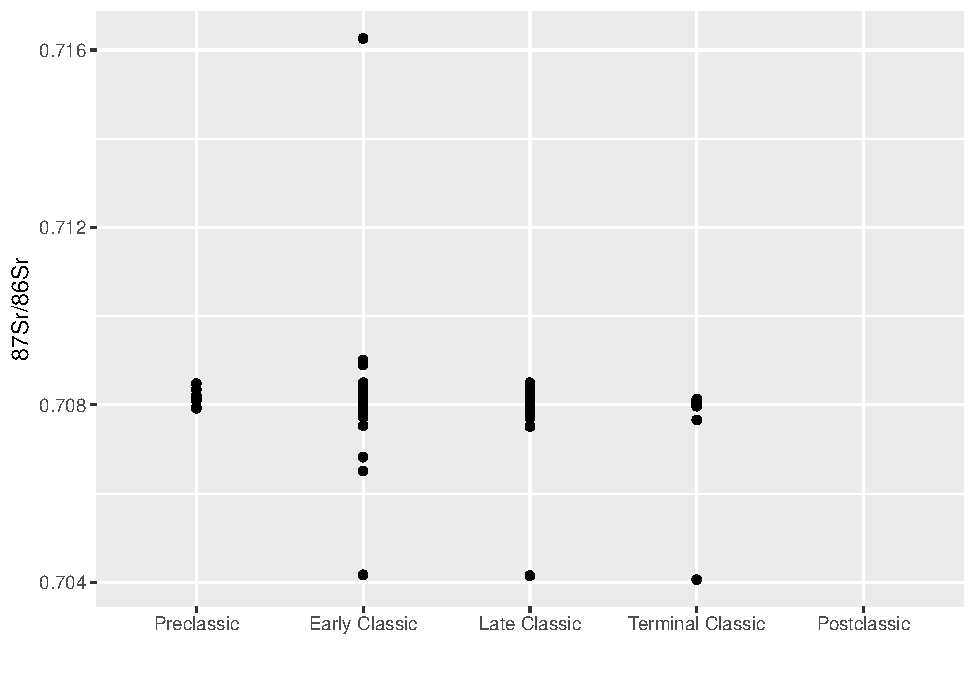
\includegraphics{img/unnamed-chunk-2-1.pdf}

Next, I examine the destriptive statistics for strontium isotope ratios
and oxygen isotope ratios. Wright provides three columns in her tables.
The first column lists all of the included data points (``Complete''),
the second removes obvious geologically distant samples (``Trimmed''),
and the third further removes outliers (``Local''), such that the
population distribution becomes a normal distribution when the
Shapiro-Wilks test is completed. I completed the first (``Complete'')
and third (``Local'') columns for her descriptive statistics. She did
not specify which outliers she removed for the Trimmed, but did specify
the parameters for the Local.

To generate Table 2. we need to create multiple piplines using the
\%\textgreater{}\% function. To get started (install if necessary and)
load the \{dplyr\},\{tidyverse\}, and \{e1071\} packages. Eacy of these
packages will help with descriptive stats. \{dplyr\} allows pipelines to
be created to stream the data together in a single file. \{e1071\}
carries the skewness and kurtosis statistics.

\begin{Shaded}
\begin{Highlighting}[]
\KeywordTok{library}\NormalTok{(dplyr)}
\KeywordTok{library}\NormalTok{(tidyverse)}
\KeywordTok{library}\NormalTok{(e1071)}
\end{Highlighting}
\end{Shaded}

\begin{verbatim}
## Warning: package 'e1071' was built under R version 3.5.3
\end{verbatim}

\begin{Shaded}
\begin{Highlighting}[]
\CommentTok{#The Mode() function in baseR tells you the class of an object. The get the mathematical mode (or the most frequent number), we have to create our own function: }

\NormalTok{Mode <-}\StringTok{ }\ControlFlowTok{function}\NormalTok{(x) \{}
    \ControlFlowTok{if}\NormalTok{ (}\KeywordTok{is.numeric}\NormalTok{(x)) \{}
\NormalTok{        x_table <-}\StringTok{ }\KeywordTok{table}\NormalTok{(x)}
        \KeywordTok{return}\NormalTok{(}\KeywordTok{as.numeric}\NormalTok{(}\KeywordTok{names}\NormalTok{(x_table)[}\KeywordTok{which.max}\NormalTok{(x_table)]))}
\NormalTok{    \}}
\NormalTok{\}}

\CommentTok{#Now we can build our descriptive statistics pipeline. }
\NormalTok{SrComplete <-}\StringTok{ }\NormalTok{d }\OperatorTok
\StringTok{  }\KeywordTok{select}\NormalTok{(X87Sr.86Sr) }\OperatorTok\StringTok{ }\CommentTok{#here I am telling R which column from my dataset to pull from}
\StringTok{  }\KeywordTok{summarise}\NormalTok{(}\DataTypeTok{mean =} \KeywordTok{mean}\NormalTok{(X87Sr.86Sr, }\DataTypeTok{na.rm =} \OtherTok{TRUE}\NormalTok{), }\CommentTok{#now I can go through and put in the statistical parameters I want}
            \DataTypeTok{sd =} \KeywordTok{sd}\NormalTok{(X87Sr.86Sr, }\DataTypeTok{na.rm =} \OtherTok{TRUE}\NormalTok{),}
            \DataTypeTok{count =} \KeywordTok{length}\NormalTok{(}\KeywordTok{na.omit}\NormalTok{(X87Sr.86Sr)),}
            \DataTypeTok{min =} \KeywordTok{min}\NormalTok{(X87Sr.86Sr, }\DataTypeTok{na.rm =} \OtherTok{TRUE}\NormalTok{), }
            \DataTypeTok{max =} \KeywordTok{max}\NormalTok{(X87Sr.86Sr, }\DataTypeTok{na.rm =} \OtherTok{TRUE}\NormalTok{),}
            \DataTypeTok{CV =} \KeywordTok{sd}\NormalTok{(X87Sr.86Sr, }\DataTypeTok{na.rm =} \OtherTok{TRUE}\NormalTok{)}\OperatorTok{/}\StringTok{ }\KeywordTok{mean}\NormalTok{(X87Sr.86Sr, }\DataTypeTok{na.rm =} \OtherTok{TRUE}\NormalTok{),}
            \DataTypeTok{skewness =} \KeywordTok{skewness}\NormalTok{(X87Sr.86Sr, }\DataTypeTok{na.rm =} \OtherTok{TRUE}\NormalTok{, }\DataTypeTok{type =} \DecValTok{3}\NormalTok{),}\CommentTok{# We are measuring skewness here to check out the relative symmetry of the distribution of data. So, we're looking the size of the two tails. A normal distribution should have a skewness of 0.}
            \DataTypeTok{kurtosis =} \KeywordTok{kurtosis}\NormalTok{(X87Sr.86Sr, }\DataTypeTok{na.rm =} \OtherTok{TRUE}\NormalTok{, }\DataTypeTok{type =} \DecValTok{3}\NormalTok{), }\CommentTok{#Kurtosis looks at the size of the two tails, collectively. If this value is larger than three, the data is not normally distributed. So, in evaluating the numbers, we are seeking to see how much of the data fall in the tails. A negative value means that the data has less in the tails than a typical distribution would. Conversely, if the kurtosis value is positive, the data has more in the tails than a normal distribution.}
            \DataTypeTok{median =} \KeywordTok{median}\NormalTok{(X87Sr.86Sr, }\DataTypeTok{na.rm =} \OtherTok{TRUE}\NormalTok{),}
            \DataTypeTok{SrMode =} \KeywordTok{Mode}\NormalTok{(X87Sr.86Sr))}

\NormalTok{SrLocal <-}\StringTok{ }\NormalTok{d }\OperatorTok
\StringTok{  }\KeywordTok{select}\NormalTok{(X87Sr.86Sr) }\OperatorTok
\StringTok{  }\KeywordTok{filter}\NormalTok{(X87Sr.86Sr }\OperatorTok{>}\StringTok{ }\FloatTok{0.70766}\NormalTok{, X87Sr.86Sr }\OperatorTok{<}\StringTok{ }\FloatTok{0.70850}\NormalTok{) }\OperatorTok\StringTok{ }\CommentTok{#here I am filtering the dataset to only count for the 'local' isotope ratios, as defined by Wright(2012)}
\StringTok{  }\KeywordTok{summarise}\NormalTok{(}\DataTypeTok{mean =} \KeywordTok{mean}\NormalTok{(X87Sr.86Sr, }\DataTypeTok{na.rm =} \OtherTok{TRUE}\NormalTok{),}
            \DataTypeTok{sd =} \KeywordTok{sd}\NormalTok{(X87Sr.86Sr, }\DataTypeTok{na.rm =} \OtherTok{TRUE}\NormalTok{),}
            \DataTypeTok{count =} \KeywordTok{length}\NormalTok{(}\KeywordTok{na.omit}\NormalTok{(X87Sr.86Sr)),}
            \DataTypeTok{min =} \KeywordTok{min}\NormalTok{(X87Sr.86Sr, }\DataTypeTok{na.rm =} \OtherTok{TRUE}\NormalTok{), }
            \DataTypeTok{max =} \KeywordTok{max}\NormalTok{(X87Sr.86Sr, }\DataTypeTok{na.rm =} \OtherTok{TRUE}\NormalTok{),}
            \DataTypeTok{CV =} \KeywordTok{sd}\NormalTok{(X87Sr.86Sr, }\DataTypeTok{na.rm =} \OtherTok{TRUE}\NormalTok{)}\OperatorTok{/}\StringTok{ }\KeywordTok{mean}\NormalTok{(X87Sr.86Sr, }\DataTypeTok{na.rm =} \OtherTok{TRUE}\NormalTok{),}
            \DataTypeTok{skewness =} \KeywordTok{skewness}\NormalTok{(X87Sr.86Sr, }\DataTypeTok{na.rm =} \OtherTok{TRUE}\NormalTok{, }\DataTypeTok{type =} \DecValTok{3}\NormalTok{),}
            \DataTypeTok{kurtosis =} \KeywordTok{kurtosis}\NormalTok{(X87Sr.86Sr, }\DataTypeTok{na.rm =} \OtherTok{TRUE}\NormalTok{, }\DataTypeTok{type =} \DecValTok{3}\NormalTok{), }
            \DataTypeTok{median =} \KeywordTok{median}\NormalTok{(X87Sr.86Sr, }\DataTypeTok{na.rm =} \OtherTok{TRUE}\NormalTok{),}
            \DataTypeTok{SrMode =} \KeywordTok{Mode}\NormalTok{(X87Sr.86Sr))}

\NormalTok{SrStats <-}\StringTok{ }\KeywordTok{rbind}\NormalTok{(SrComplete, SrLocal)}
\NormalTok{SrStats}
\end{Highlighting}
\end{Shaded}

\begin{verbatim}
## # A tibble: 2 x 10
##    mean       sd count   min   max       CV skewness kurtosis median SrMode
##   <dbl>    <dbl> <int> <dbl> <dbl>    <dbl>    <dbl>    <dbl>  <dbl>  <dbl>
## 1 0.708 0.00113     97 0.704 0.716 0.00160     2.61    29.8    0.708  0.708
## 2 0.708 0.000179    83 0.708 0.708 0.000253   -0.281   -0.532  0.708  0.708
\end{verbatim}

I couldn't figure out how to sync up my dplyr tables with the
Shapiro-Wilk test, so I'm just doing them separately. Sorry!

\begin{Shaded}
\begin{Highlighting}[]
\NormalTok{SrCompShapiro <-}\StringTok{ }\KeywordTok{shapiro.test}\NormalTok{(d}\OperatorTok{$}\NormalTok{X87Sr.86Sr)}
\NormalTok{SrLocalShapio <-}\StringTok{ }\KeywordTok{shapiro.test}\NormalTok{(d}\OperatorTok{$}\NormalTok{X87Sr.86Sr)}

\NormalTok{SrShapiro <-}\StringTok{ }\KeywordTok{rbind}\NormalTok{(SrCompShapiro, SrLocalShapio)}
\NormalTok{SrShapiro}
\end{Highlighting}
\end{Shaded}

\begin{verbatim}
##               statistic p.value      method                       
## SrCompShapiro 0.4465441 2.081253e-17 "Shapiro-Wilk normality test"
## SrLocalShapio 0.4465441 2.081253e-17 "Shapiro-Wilk normality test"
##               data.name     
## SrCompShapiro "d$X87Sr.86Sr"
## SrLocalShapio "d$X87Sr.86Sr"
\end{verbatim}

Table 3. Canines and Molars (Repeat code from Table 2. However, use the
Average.d18o.Canines and Average.d18o.Molars columns from the dataset)

\begin{Shaded}
\begin{Highlighting}[]
\NormalTok{CaninesComplete <-}\StringTok{ }\NormalTok{d }\OperatorTok
\StringTok{  }\KeywordTok{select}\NormalTok{(Average.18O.canines) }\OperatorTok
\StringTok{  }\KeywordTok{summarise}\NormalTok{(}\DataTypeTok{mean =} \KeywordTok{mean}\NormalTok{(Average.18O.canines, }\DataTypeTok{na.rm =} \OtherTok{TRUE}\NormalTok{),}
            \DataTypeTok{sd =} \KeywordTok{sd}\NormalTok{(Average.18O.canines, }\DataTypeTok{na.rm =} \OtherTok{TRUE}\NormalTok{),}
            \DataTypeTok{count =} \KeywordTok{length}\NormalTok{(}\KeywordTok{na.omit}\NormalTok{(Average.18O.canines)),}
            \DataTypeTok{min =} \KeywordTok{min}\NormalTok{(Average.18O.canines, }\DataTypeTok{na.rm =} \OtherTok{TRUE}\NormalTok{), }
            \DataTypeTok{max =} \KeywordTok{max}\NormalTok{(Average.18O.canines, }\DataTypeTok{na.rm =} \OtherTok{TRUE}\NormalTok{),}
            \DataTypeTok{CV =} \KeywordTok{sd}\NormalTok{(Average.18O.canines, }\DataTypeTok{na.rm =} \OtherTok{TRUE}\NormalTok{)}\OperatorTok{/}\StringTok{ }\KeywordTok{mean}\NormalTok{(Average.18O.canines, }\DataTypeTok{na.rm =} \OtherTok{TRUE}\NormalTok{),}
            \DataTypeTok{skewness =} \KeywordTok{skewness}\NormalTok{(Average.18O.canines, }\DataTypeTok{na.rm =} \OtherTok{TRUE}\NormalTok{, }\DataTypeTok{type =} \DecValTok{3}\NormalTok{),}
            \DataTypeTok{kurtosis =} \KeywordTok{kurtosis}\NormalTok{(Average.18O.canines, }\DataTypeTok{na.rm =} \OtherTok{TRUE}\NormalTok{, }\DataTypeTok{type =} \DecValTok{3}\NormalTok{), }
            \DataTypeTok{median =} \KeywordTok{median}\NormalTok{(Average.18O.canines, }\DataTypeTok{na.rm =} \OtherTok{TRUE}\NormalTok{),}
            \DataTypeTok{O_Mode =} \KeywordTok{Mode}\NormalTok{(Average.18O.canines))}

\NormalTok{MolarsComplete <-}\StringTok{ }\NormalTok{d }\OperatorTok
\StringTok{  }\KeywordTok{select}\NormalTok{(Average.18O.molars) }\OperatorTok
\StringTok{  }\KeywordTok{summarise}\NormalTok{(}\DataTypeTok{mean =} \KeywordTok{mean}\NormalTok{(Average.18O.molars, }\DataTypeTok{na.rm =} \OtherTok{TRUE}\NormalTok{),}
            \DataTypeTok{sd =} \KeywordTok{sd}\NormalTok{(Average.18O.molars, }\DataTypeTok{na.rm =} \OtherTok{TRUE}\NormalTok{),}
            \DataTypeTok{count =} \KeywordTok{length}\NormalTok{(}\KeywordTok{na.omit}\NormalTok{(Average.18O.molars)),}
            \DataTypeTok{min =} \KeywordTok{min}\NormalTok{(Average.18O.molars, }\DataTypeTok{na.rm =} \OtherTok{TRUE}\NormalTok{), }
            \DataTypeTok{max =} \KeywordTok{max}\NormalTok{(Average.18O.molars, }\DataTypeTok{na.rm =} \OtherTok{TRUE}\NormalTok{),}
            \DataTypeTok{CV =} \KeywordTok{sd}\NormalTok{(Average.18O.molars, }\DataTypeTok{na.rm =} \OtherTok{TRUE}\NormalTok{)}\OperatorTok{/}\StringTok{ }\KeywordTok{mean}\NormalTok{(Average.18O.molars, }\DataTypeTok{na.rm =} \OtherTok{TRUE}\NormalTok{),}
            \DataTypeTok{skewness =} \KeywordTok{skewness}\NormalTok{(Average.18O.molars, }\DataTypeTok{na.rm =} \OtherTok{TRUE}\NormalTok{, }\DataTypeTok{type =} \DecValTok{3}\NormalTok{),}
            \DataTypeTok{kurtosis =} \KeywordTok{kurtosis}\NormalTok{(Average.18O.molars, }\DataTypeTok{na.rm =} \OtherTok{TRUE}\NormalTok{, }\DataTypeTok{type =} \DecValTok{3}\NormalTok{), }
            \DataTypeTok{median =} \KeywordTok{median}\NormalTok{(Average.18O.molars, }\DataTypeTok{na.rm =} \OtherTok{TRUE}\NormalTok{),}
            \DataTypeTok{O_Mode =} \KeywordTok{Mode}\NormalTok{(Average.18O.molars))}

\NormalTok{OxygenStats <-}\StringTok{ }\KeywordTok{rbind}\NormalTok{(CaninesComplete, MolarsComplete)}
\NormalTok{OxygenStats}
\end{Highlighting}
\end{Shaded}

\begin{verbatim}
## # A tibble: 2 x 10
##    mean    sd count   min   max     CV skewness kurtosis median O_Mode
##   <dbl> <dbl> <int> <dbl> <dbl>  <dbl>    <dbl>    <dbl>  <dbl>  <dbl>
## 1 -2.88  1.03    90  -5.9  -1   -0.360   -0.466   -0.246   -2.8   -2.8
## 2 -3.09  1.35    63  -6.7  -0.1 -0.437   -0.607    0.144   -2.8   -2.4
\end{verbatim}

\begin{Shaded}
\begin{Highlighting}[]
\NormalTok{CanineShapiro <-}\StringTok{ }\KeywordTok{shapiro.test}\NormalTok{(d}\OperatorTok{$}\NormalTok{Average.18O.canines)}
\NormalTok{MolarShapiro <-}\StringTok{ }\KeywordTok{shapiro.test}\NormalTok{(d}\OperatorTok{$}\NormalTok{Average.18O.molars)}
\NormalTok{OShapiro <-}\StringTok{ }\KeywordTok{rbind}\NormalTok{(CanineShapiro, MolarShapiro)}
\NormalTok{OShapiro}
\end{Highlighting}
\end{Shaded}

\begin{verbatim}
##               statistic p.value    method                       
## CanineShapiro 0.9762621 0.09837046 "Shapiro-Wilk normality test"
## MolarShapiro  0.9540207 0.0194777  "Shapiro-Wilk normality test"
##               data.name              
## CanineShapiro "d$Average.18O.canines"
## MolarShapiro  "d$Average.18O.molars"
\end{verbatim}

Fig. 4 is two histograms comparing the distributions of averages of d18O
from canines and molars with a normal distribution line plotted over
them. We can use \{ggplot2\} for shortened code. Note: I'm still not
sure why my distribution lines a plotting so small.

\begin{Shaded}
\begin{Highlighting}[]
\KeywordTok{ggplot}\NormalTok{(}\DataTypeTok{data =}\NormalTok{ d, }\KeywordTok{aes}\NormalTok{(d}\OperatorTok{$}\NormalTok{Average.18O.canines)) }\OperatorTok{+}\StringTok{ }\CommentTok{#tells us our data to pull from}
\StringTok{  }\KeywordTok{geom_histogram}\NormalTok{(}\DataTypeTok{na.rm =} \OtherTok{TRUE}\NormalTok{, }\CommentTok{#which type of plot we'll be using and the parameters}
                 \DataTypeTok{breaks =} \KeywordTok{seq}\NormalTok{(}\OperatorTok{-}\DecValTok{7}\NormalTok{, }\DecValTok{0}\NormalTok{, }\DataTypeTok{by =} \FloatTok{0.5}\NormalTok{), }\CommentTok{#I've used binwidth() and bins() along with breaks() to make my bins fall on whole numbers. If I don't use breaks() then the histogram plots on half numbers for the x-axis tick marks, rather than whole numbers. }
                 \DataTypeTok{binwidth =} \FloatTok{0.5}\NormalTok{,}
                 \DataTypeTok{bins =} \DecValTok{15}\NormalTok{,}
                 \DataTypeTok{col =} \StringTok{"blue"}\NormalTok{,}
                 \DataTypeTok{fill =} \StringTok{"red"}\NormalTok{, }
                 \DataTypeTok{probability =} \OtherTok{FALSE}\NormalTok{) }\OperatorTok{+}
\StringTok{  }\KeywordTok{geom_density}\NormalTok{(}\DataTypeTok{col=} \StringTok{"green"}\NormalTok{) }\OperatorTok{+}\StringTok{ }\CommentTok{#this creates the normal distribution line. }
\StringTok{  }\KeywordTok{labs}\NormalTok{(}\DataTypeTok{x =} \StringTok{"Canine Average"}\OperatorTok{~}\NormalTok{delta}\OperatorTok{*}\StringTok{'18O(\textbackslash{}u2030PDB)'}\NormalTok{, }\DataTypeTok{y =} \StringTok{"Frequency"}\NormalTok{) }\OperatorTok{+}
\StringTok{  }\KeywordTok{xlim}\NormalTok{(}\KeywordTok{c}\NormalTok{(}\OperatorTok{-}\FloatTok{7.0}\NormalTok{, }\FloatTok{0.0}\NormalTok{)) }\OperatorTok{+}\StringTok{ }
\StringTok{  }\KeywordTok{ylim}\NormalTok{(}\KeywordTok{c}\NormalTok{(}\DecValTok{0}\NormalTok{,}\DecValTok{20}\NormalTok{)) }
\end{Highlighting}
\end{Shaded}

\begin{verbatim}
## Warning: Ignoring unknown parameters: probability
\end{verbatim}

\begin{verbatim}
## Warning: Removed 44 rows containing non-finite values (stat_density).
\end{verbatim}

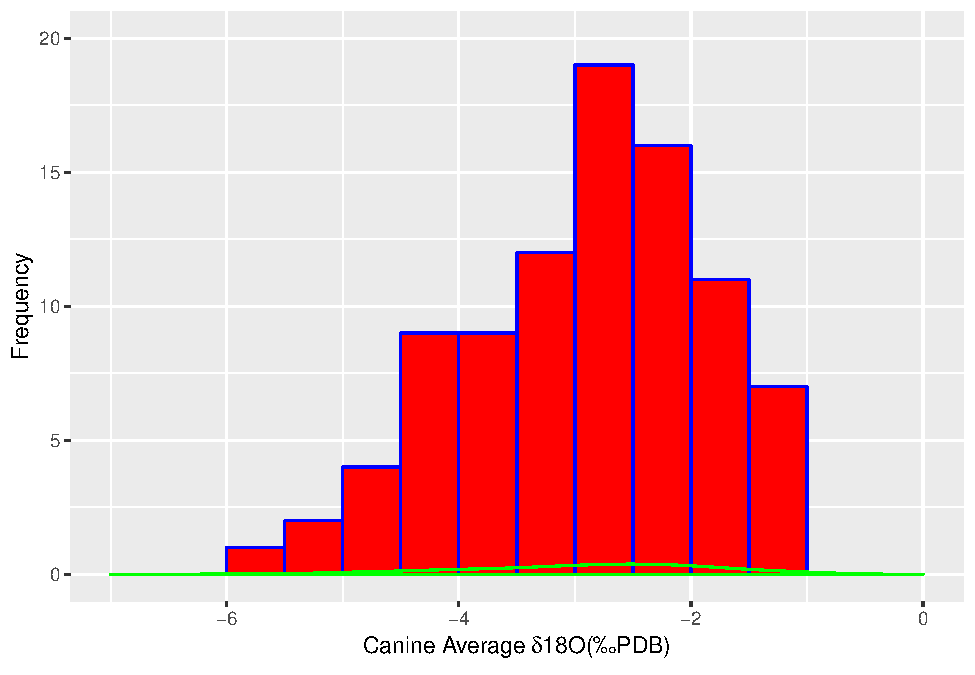
\includegraphics{img/unnamed-chunk-7-1.pdf}

\begin{Shaded}
\begin{Highlighting}[]
\KeywordTok{ggplot}\NormalTok{(}\DataTypeTok{data =}\NormalTok{ d, }\KeywordTok{aes}\NormalTok{(d}\OperatorTok{$}\NormalTok{Average.18O.molars)) }\OperatorTok{+}\StringTok{ }
\StringTok{  }\KeywordTok{geom_histogram}\NormalTok{(}\DataTypeTok{na.rm =} \OtherTok{TRUE}\NormalTok{,}
                 \DataTypeTok{breaks =} \KeywordTok{seq}\NormalTok{(}\OperatorTok{-}\DecValTok{7}\NormalTok{, }\DecValTok{0}\NormalTok{, }\DataTypeTok{by =} \FloatTok{0.5}\NormalTok{),}
                 \DataTypeTok{binwidth =} \FloatTok{0.5}\NormalTok{,}
                 \DataTypeTok{bins =} \DecValTok{10}\NormalTok{,}
                 \DataTypeTok{col =} \StringTok{"blue"}\NormalTok{,}
                 \DataTypeTok{fill =} \StringTok{"red"}\NormalTok{,}
                 \DataTypeTok{probability =} \OtherTok{FALSE}\NormalTok{) }\OperatorTok{+}
\StringTok{  }\KeywordTok{geom_density}\NormalTok{(}\DataTypeTok{col=}\StringTok{"green"}\NormalTok{) }\OperatorTok{+}
\StringTok{  }\KeywordTok{labs}\NormalTok{(}\DataTypeTok{x =} \StringTok{"Third Molar Average"}\OperatorTok{~}\NormalTok{delta}\OperatorTok{*}\StringTok{'18O(\textbackslash{}u2030PDB)'}\NormalTok{, }\DataTypeTok{y =} \StringTok{"Frequency"}\NormalTok{) }\OperatorTok{+}\StringTok{ }\CommentTok{#Note: the \textbackslash{}u2030 is code for the permille symbol. ~delta* notes that there should be a space after "Average", then a small delta symbol with no space between it and the 18. }
\StringTok{  }\KeywordTok{xlim}\NormalTok{(}\KeywordTok{c}\NormalTok{(}\OperatorTok{-}\FloatTok{7.0}\NormalTok{, }\FloatTok{0.0}\NormalTok{)) }\OperatorTok{+}\StringTok{ }
\StringTok{  }\KeywordTok{ylim}\NormalTok{(}\KeywordTok{c}\NormalTok{(}\DecValTok{0}\NormalTok{,}\DecValTok{12}\NormalTok{))}
\end{Highlighting}
\end{Shaded}

\begin{verbatim}
## Warning: Ignoring unknown parameters: probability
\end{verbatim}

\begin{verbatim}
## Warning: Removed 71 rows containing non-finite values (stat_density).
\end{verbatim}

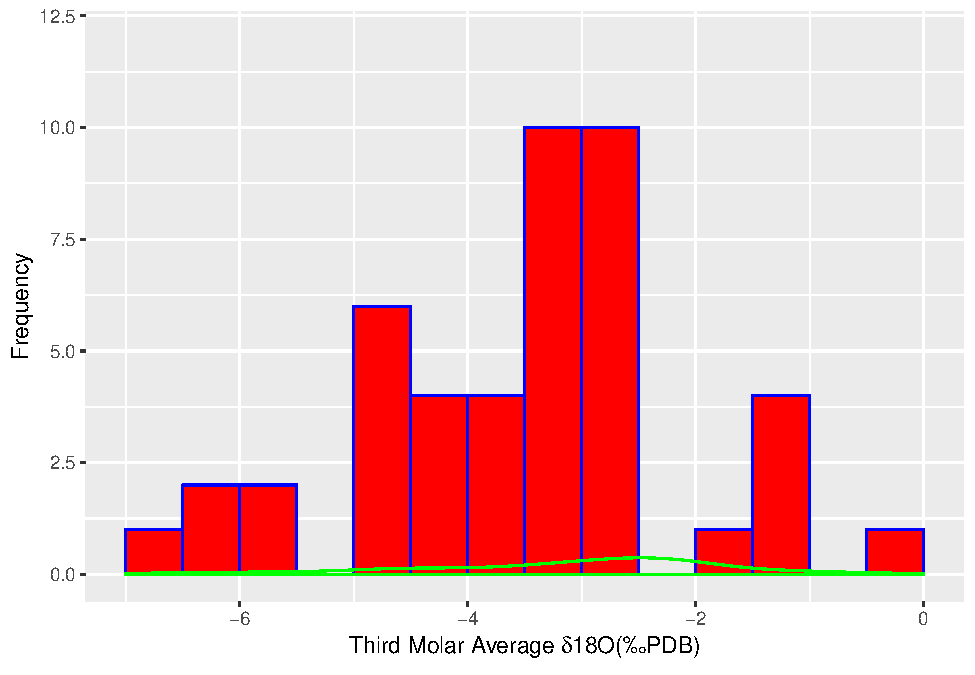
\includegraphics{img/unnamed-chunk-7-2.pdf}

Fig. 5 = QQ Plots of oxygen isotope data using \{ggplot2\}

\begin{Shaded}
\begin{Highlighting}[]
\NormalTok{qc <-}\StringTok{ }\KeywordTok{ggplot}\NormalTok{(d, }\KeywordTok{aes}\NormalTok{(}\DataTypeTok{sample =}\NormalTok{ d}\OperatorTok{$}\NormalTok{Average.18O.canines)) }\OperatorTok{+}\StringTok{ }\CommentTok{#tells us which data to pull from}
\StringTok{  }\KeywordTok{stat_qq}\NormalTok{() }\OperatorTok{+}\StringTok{ }\CommentTok{#type of plot}
\StringTok{  }\KeywordTok{stat_qq_line}\NormalTok{() }\OperatorTok{+}\StringTok{ }\CommentTok{#adds the expected line}
\StringTok{  }\KeywordTok{labs}\NormalTok{(}\DataTypeTok{title =} \StringTok{"Canine QQ"}\NormalTok{)}

\NormalTok{qm <-}\StringTok{ }\KeywordTok{ggplot}\NormalTok{(d, }\KeywordTok{aes}\NormalTok{(}\DataTypeTok{sample =}\NormalTok{ d}\OperatorTok{$}\NormalTok{Average.18O.molars)) }\OperatorTok{+}
\StringTok{  }\KeywordTok{stat_qq}\NormalTok{() }\OperatorTok{+}
\StringTok{  }\KeywordTok{stat_qq_line}\NormalTok{() }\OperatorTok{+}
\StringTok{  }\KeywordTok{labs}\NormalTok{(}\DataTypeTok{title =} \StringTok{"Molars QQ"}\NormalTok{)}

\NormalTok{qc}
\end{Highlighting}
\end{Shaded}

\begin{verbatim}
## Warning: Removed 44 rows containing non-finite values (stat_qq).
\end{verbatim}

\begin{verbatim}
## Warning: Removed 44 rows containing non-finite values (stat_qq_line).
\end{verbatim}

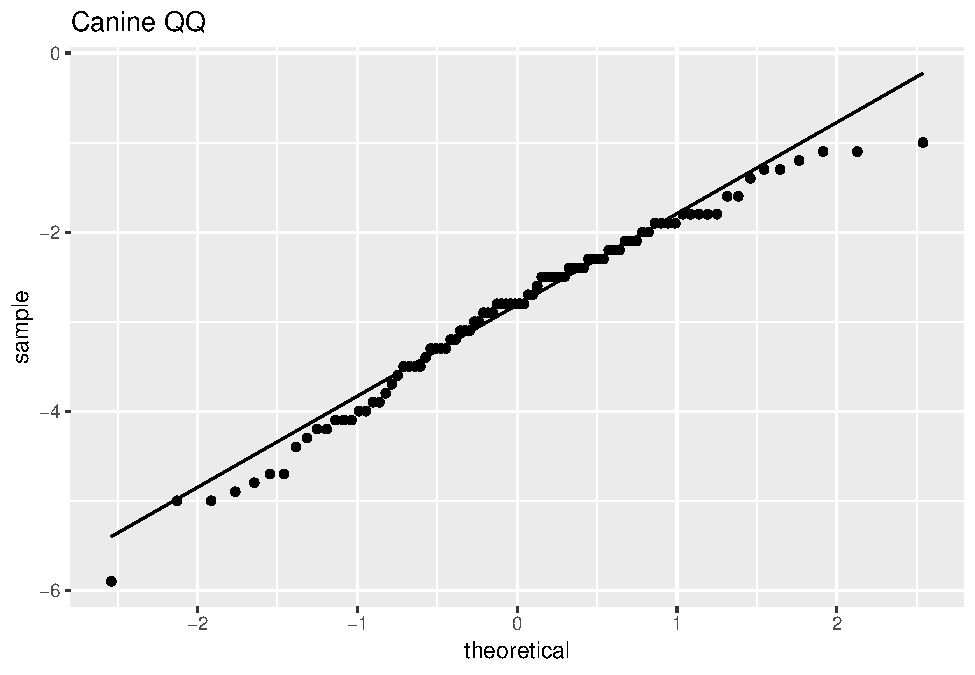
\includegraphics{img/unnamed-chunk-8-1.pdf}

\begin{Shaded}
\begin{Highlighting}[]
\NormalTok{qm}
\end{Highlighting}
\end{Shaded}

\begin{verbatim}
## Warning: Removed 71 rows containing non-finite values (stat_qq).
\end{verbatim}

\begin{verbatim}
## Warning: Removed 71 rows containing non-finite values (stat_qq_line).
\end{verbatim}

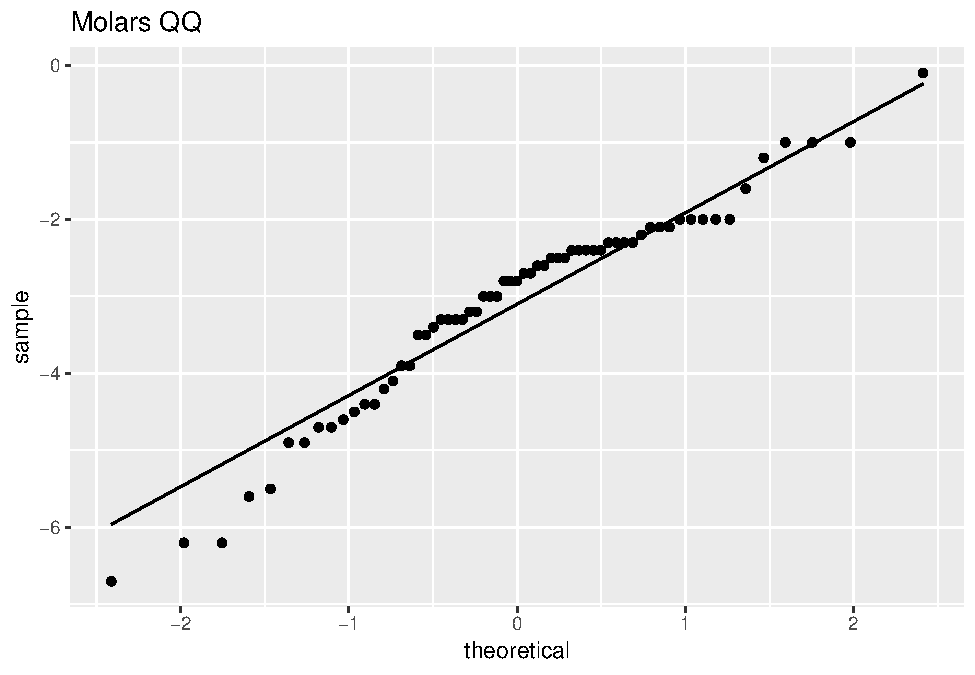
\includegraphics{img/unnamed-chunk-8-2.pdf}

Fig. 6 Finally, We will plot a multivariate scatterplot comparing
strontium isotope ratios to oxygen isotope ratios using \{ggplot2\}

\begin{Shaded}
\begin{Highlighting}[]
\KeywordTok{library}\NormalTok{(ggplot2) }\CommentTok{#load in the \{ggplot2\} package}
\NormalTok{sro <-}\StringTok{ }\KeywordTok{ggplot}\NormalTok{(d, }\KeywordTok{aes}\NormalTok{(}\DataTypeTok{x =}\NormalTok{ d}\OperatorTok{$}\NormalTok{X87Sr.86Sr, }\DataTypeTok{y =}\NormalTok{ d}\OperatorTok{$}\NormalTok{Average.18O.canines, d}\OperatorTok{$}\NormalTok{Average.18O.molars), }\KeywordTok{colours}\NormalTok{(}\DataTypeTok{distinct =} \OtherTok{TRUE}\NormalTok{)) }\OperatorTok{+}\StringTok{ }\CommentTok{# Data tells you which file to pull from; aes lets you set up your x,y plot.                           }
\StringTok{  }\KeywordTok{geom_point}\NormalTok{(}\DataTypeTok{na.rm =} \OtherTok{TRUE}\NormalTok{) }\OperatorTok{+}\StringTok{ }
\StringTok{  }\KeywordTok{xlab}\NormalTok{(}\StringTok{"87Sr/86Sr"}\NormalTok{) }\OperatorTok{+}\StringTok{ }\KeywordTok{ylab}\NormalTok{(}\StringTok{'d18O(\textbackslash{}u2030PDB)'}\NormalTok{)}
\NormalTok{sro  }\CommentTok{# and, finally, we plot}
\end{Highlighting}
\end{Shaded}

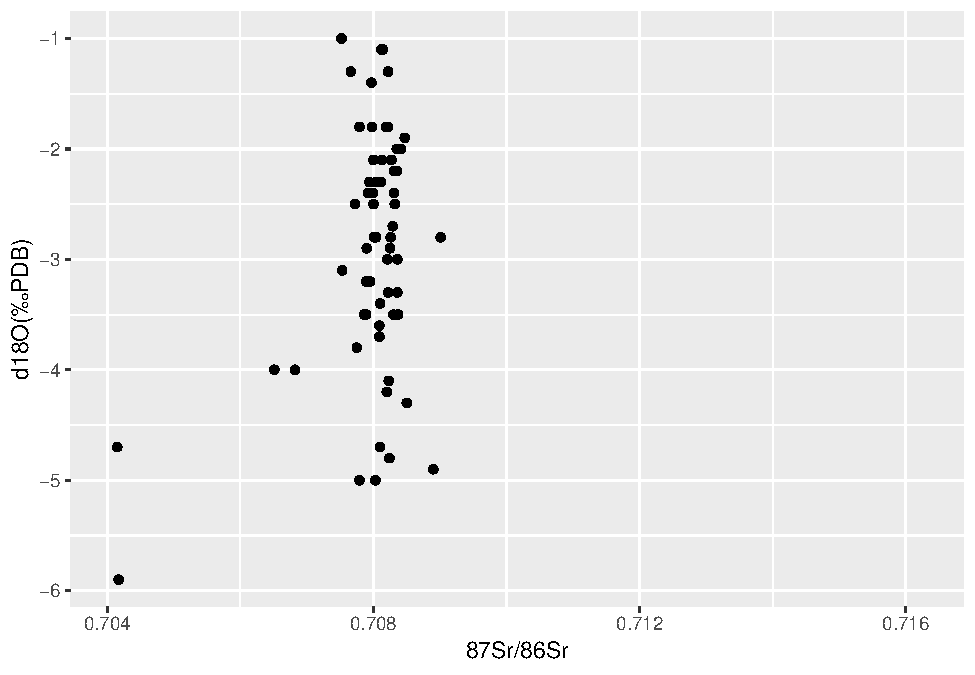
\includegraphics{img/unnamed-chunk-9-1.pdf}

\subsection{Summary}\label{summary}

Summary statistics using \{dplyr\}: summarise(), filter(),
\%\textgreater{}\%

Data Normality Checks: Shapiro.Wilks Testing, Skewness, Kurtosis, QQ
Plots

Plotting histograms with normal distribution lines usins \{ggplot2\}:
ggplot(data = , aes(x,y)) + geom\_histogram + geom\_density()\ldots{}

Plotting QQ plots with \{ggplot2\}: ggplot(data = , aes(sample = )) +
stat\_qq() + stat\_qq\_line() + labs()\ldots{}

Generating a scatterplot with \{ggplot2\}: ggplot(data = , aes(x, y)) +
geom\_point + xlab + ylab\ldots{}

\subsection{References}\label{references}

\url{https://blog.exploratory.io/filter-data-with-dplyr-76cf5f1a258e}

dplyr cheatsheet: \url{https://www.rstudio.com/resources/cheatsheets/}

ggplot2 cheatsheet: \url{https://www.rstudio.com/resources/cheatsheets/}

Kabacoff, Robert I.2011. \emph{R in Action: Data Analysis and Graphics
with R} Manning Publications: Shelter Island, NY.\\
\url{https://ggplot2.tidyverse.org/reference/geom_qq.html}


\end{document}
